% =====================================================================
%  Capítulo 16. Estudios de eventos
% =====================================================================
\chapter[Estudios de eventos]{Estudios de eventos: rendimientos anormales, pruebas y sus trampas}\label{cap:eventos}

\section*{Objetivos de aprendizaje}
Al terminar este capítulo, el lector podrá:
\begin{enumerate}[label=\arabic*.,leftmargin=*]
  \item Diseñar un estudio de eventos: fecha del evento, ventanas de estimación y del evento, y modelo de rendimiento
        normal.
  \item Calcular rendimientos anormales y acumulados con su varianza exacta, incluido el error de estimación, y
        demostrar su equivalencia con una regresión con variables ficticias.
  \item Agregar muchos eventos y aplicar las pruebas paramétricas ($J_1$, Patell, Boehmer-Musumeci-Poulsen) y no
        paramétricas (signo y rangos de Corrado).
  \item Reconocer las dos trampas más comunes, los eventos simultáneos y la varianza inducida por el evento, y medir
        con simulaciones el tamaño y la potencia de cada prueba.
\end{enumerate}

\section*{Motivación}
El 25 de julio de 2018, después del cierre, Facebook publicó sus resultados del segundo trimestre. Al día siguiente su
acción cayó cerca de 19\,\%, la mayor pérdida de valor de mercado de una empresa estadounidense en un solo día hasta ese
momento. ¿Cuánto de esa caída se debe al anuncio y cuánto al mercado? ¿Es estadísticamente distinta de un mal día
cualquiera? El estudio de eventos, formalizado por Fama, Fisher, Jensen y Roll (1969), responde estas preguntas comparando el
rendimiento observado con el que se habría esperado sin el evento. Es probablemente la herramienta empírica más usada
en finanzas corporativas, en derecho (para cuantificar daños en litigios de valores) y en la evaluación de políticas,
como los anuncios de un banco central.

\paragraph{Datos del capítulo.} Precios de cierre diarios ajustados de Apple (AAPL), Amazon (AMZN), Facebook (FB) y
Alphabet (GOOG), de enero de 2014 a diciembre de 2018, y el índice S\&P 500 en las mismas fechas (1\,257 rendimientos
diarios). Para los anuncios de política monetaria usamos el S\&P 500 desde 1999, el índice de volatilidad VIX y las 40
fechas de las reuniones programadas del Comité Federal de Mercado Abierto (FOMC) de 2014 a 2018, tomadas de las páginas
históricas de la Reserva Federal. Los rendimientos son simples y en porcentaje.

% ---------------------------------------------------------------------
\section{El diseño de un estudio de eventos}
% ---------------------------------------------------------------------

Un estudio de eventos mide el tiempo en días hábiles relativos al evento, $\tau$. El día 0 es el primer día en que el
mercado pudo reaccionar: si la noticia sale después del cierre, como los resultados de Facebook, el día 0 es el día
hábil siguiente. Se definen dos ventanas (Figura~\ref{fig:lineatiempo}):
\begin{itemize}[leftmargin=*]
  \item la \emph{ventana de estimación}, de $L_1$ días antes del evento, donde se estima cómo se comporta el activo en
        condiciones normales; en este capítulo, $\tau=-250,\dots,-11$, con $L_1=240$;
  \item la \emph{ventana del evento}, de $L_2$ días alrededor del día 0, donde se mide el efecto; aquí,
        $\tau=-5,\dots,+5$, con $L_2=11$.
\end{itemize}
El espacio entre ambas ($\tau=-10,\dots,-6$) evita que una filtración previa al anuncio contamine la estimación.

\begin{figure}[ht]
\centering
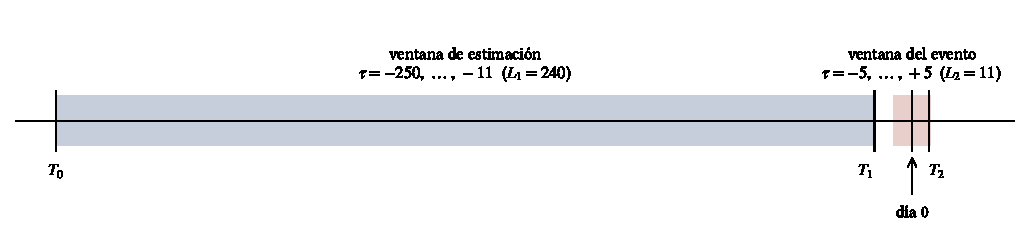
\includegraphics[width=\linewidth]{graficos/cap16_fig_linea_tiempo.pdf}
\caption{Línea de tiempo de un estudio de eventos con las ventanas usadas en el capítulo.}
\label{fig:lineatiempo}
\end{figure}

\begin{definicion}[Rendimiento anormal]
El rendimiento anormal del activo $i$ en el día $\tau$ es la diferencia entre el rendimiento observado y el rendimiento
normal estimado, $AR_{i\tau}=R_{i\tau}-\hat\E[R_{i\tau}\mid\text{sin evento}]$. El rendimiento anormal acumulado entre
$\tau_1$ y $\tau_2$ es $CAR_i(\tau_1,\tau_2)=\sum_{\tau=\tau_1}^{\tau_2}AR_{i\tau}$.
\end{definicion}

Los tres modelos de rendimiento normal más usados son:
\begin{itemize}[leftmargin=*]
  \item \textbf{media constante}: $R_{i\tau}=\mu_i+\varepsilon_{i\tau}$, de modo que $AR_{i\tau}=R_{i\tau}-\bar R_i$;
  \item \textbf{ajustado por mercado}: $AR_{i\tau}=R_{i\tau}-R_{m\tau}$, sin parámetros que estimar (equivale a fijar
        $\alpha=0$ y $\beta=1$);
  \item \textbf{modelo de mercado}: $R_{i\tau}=\alpha_i+\beta_iR_{m\tau}+\varepsilon_{i\tau}$, estimado por MCO en la
        ventana de estimación, de modo que $AR_{i\tau}=R_{i\tau}-\hat\alpha_i-\hat\beta_iR_{m\tau}$.
\end{itemize}
El modelo de mercado quita la parte del rendimiento que explica el mercado, lo que reduce la varianza del rendimiento
anormal tanto más cuanto mayor es el $R^2$ de la regresión. Pueden usarse modelos de factores (Capítulo~\ref{cap:factores}),
pero con datos diarios la ganancia sobre el modelo de mercado suele ser pequeña (MacKinlay, 1997).

% ---------------------------------------------------------------------
\section{La varianza de los rendimientos anormales}
% ---------------------------------------------------------------------

\begin{proposicion}[Varianza del rendimiento anormal]\label{prop:varar}
Sea el modelo de mercado con errores i.i.d.\ de varianza $\sigma^2$, independientes del mercado, estimado con $L_1$
observaciones. Sean $\hat\mu_m$ la media del mercado en la ventana de estimación y
$S_{mm}=\sum_{t}(R_{mt}-\hat\mu_m)^2$. Si no hay evento, condicionado en los rendimientos del mercado,
\[
  \E[AR_{i\tau}]=0,\qquad
  \Var(AR_{i\tau})=\sigma^2\Bigl[1+\frac1{L_1}+\frac{(R_{m\tau}-\hat\mu_m)^2}{S_{mm}}\Bigr].
\]
\end{proposicion}

\begin{proof}
Sin evento, $R_{i\tau}=\alpha_i+\beta_iR_{m\tau}+\varepsilon_{i\tau}$. Restamos el rendimiento normal estimado:
\begin{align*}
  AR_{i\tau} &= \alpha_i+\beta_iR_{m\tau}+\varepsilon_{i\tau}-\hat\alpha_i-\hat\beta_iR_{m\tau}\\
             &= \varepsilon_{i\tau}-\bigl[(\hat\alpha_i-\alpha_i)+(\hat\beta_i-\beta_i)R_{m\tau}\bigr].
\end{align*}
Los estimadores de MCO son insesgados, así que $\E[AR_{i\tau}]=0$. El término entre corchetes es el error de estimar la
recta en el punto $R_{m\tau}$. Depende solo de los errores de la ventana de estimación, que son independientes de
$\varepsilon_{i\tau}$; por tanto, las varianzas se suman. Escribiendo la recta en forma centrada,
$\hat\alpha_i+\hat\beta_ix=\bar R_i+\hat\beta_i(x-\hat\mu_m)$, donde $\bar R_i$ y $\hat\beta_i$ no están correlacionados:
\begin{align*}
  \Var(AR_{i\tau}) &= \Var(\varepsilon_{i\tau})+\Var\bigl(\bar R_i+\hat\beta_i(R_{m\tau}-\hat\mu_m)\bigr)\\
                   &= \sigma^2+\Var(\bar R_i)+(R_{m\tau}-\hat\mu_m)^2\Var(\hat\beta_i)\\
                   &= \sigma^2+\frac{\sigma^2}{L_1}+(R_{m\tau}-\hat\mu_m)^2\,\frac{\sigma^2}{S_{mm}}\\
                   &= \sigma^2\Bigl[1+\frac1{L_1}+\frac{(R_{m\tau}-\hat\mu_m)^2}{S_{mm}}\Bigr].
\end{align*}
\end{proof}

El primer término es la varianza del error del día del evento; los otros dos son el costo de no conocer $\alpha_i$ y
$\beta_i$. Con $L_1=240$ el segundo es $1/240=0{,}0042$, y el tercero es grande solo en días en que el mercado se movió mucho.
En forma matricial, si $X$ ($L_1\times2$) tiene las filas $(1,R_{mt})$ de la ventana de estimación y $X^*$ ($L_2\times2$) las
de la ventana del evento, el vector $\mathbf{AR}_i$ tiene covarianza
\[
  V_i=\sigma^2\bigl[I_{L_2}+X^*(X'X)^{-1}X^{*\prime}\bigr].
\]
Los elementos fuera de la diagonal no son cero: todos los $AR$ comparten el mismo error de estimación.

\begin{corolario}[Varianza del CAR]\label{cor:varcar}
Con $\boldsymbol\gamma$ el vector de unos en los días $\tau_1,\dots,\tau_2$ y ceros en el resto, $CAR_i=\boldsymbol\gamma'\mathbf{AR}_i$ y
\[
  \Var(CAR_i)=\boldsymbol\gamma'V_i\boldsymbol\gamma=\sigma^2\bigl[(\tau_2-\tau_1+1)+\boldsymbol\gamma'X^*(X'X)^{-1}X^{*\prime}\boldsymbol\gamma\bigr].
\]
\end{corolario}

\begin{proof}
Es la varianza de una combinación lineal:
\begin{align*}
  \Var(\boldsymbol\gamma'\mathbf{AR}_i) &= \boldsymbol\gamma'V_i\boldsymbol\gamma\\
                                        &= \sigma^2\boldsymbol\gamma'I\boldsymbol\gamma+\sigma^2\boldsymbol\gamma'X^*(X'X)^{-1}X^{*\prime}\boldsymbol\gamma\\
                                        &= \sigma^2(\tau_2-\tau_1+1)+\sigma^2\boldsymbol\gamma'X^*(X'X)^{-1}X^{*\prime}\boldsymbol\gamma,
\end{align*}
porque $\boldsymbol\gamma'\boldsymbol\gamma$ cuenta los unos de $\boldsymbol\gamma$.
\end{proof}

En la práctica se sustituye $\sigma^2$ por $s^2=\sum\hat\varepsilon_t^2/(L_1-2)$. Con errores normales, el cociente
$AR_{i\tau}/\sqrt{\hat V_{i,\tau\tau}}$ sigue una $t$ de Student con $L_1-2$ grados de libertad, y lo mismo el
$CAR$ estandarizado.

\begin{proposicion}[El rendimiento anormal como coeficiente de una ficticia]\label{prop:ficticia}
Agregue a la ventana de estimación la observación del día $\tau$ y estime por MCO
$R_{it}=\alpha_i+\beta_iR_{mt}+\delta\,D_t+u_t$, con $D_t=1$ solo en el día $\tau$. Entonces $\hat\delta=AR_{i\tau}$ y su error
estándar de MCO es exactamente $\sqrt{\hat V_{i,\tau\tau}}$ de la Proposición~\ref{prop:varar}.
\end{proposicion}

\begin{proof}
La ficticia solo actúa en el día $\tau$, así que $\hat\delta$ puede ajustar esa observación sin error y MCO lo hace: el
residuo del día $\tau$ es cero. Los demás residuos dependen solo de $(\hat\alpha_i,\hat\beta_i)$, que por tanto son los de la ventana
de estimación. Con $\mathbf x_\tau=(1,R_{m\tau})'$, la ecuación del día $\tau$ da
\begin{align*}
  R_{i\tau} &= \mathbf x_\tau'\hat{\mathbf b}+\hat\delta\\
  \hat\delta  &= R_{i\tau}-\mathbf x_\tau'\hat{\mathbf b}\\
             &= AR_{i\tau}.
\end{align*}
La suma de residuos al cuadrado es la de la ventana de estimación y los grados de libertad son $(L_1+1)-3=L_1-2$: la
estimación $s^2$ coincide. Falta el elemento de $(Z'Z)^{-1}$ que corresponde a $\delta$. Por la inversa de una matriz
particionada, es $1/(\mathbf d'M\mathbf d)$, donde $M$ es el aniquilador de las columnas $(1,R_m)$ en las $L_1+1$ observaciones.
Con $A=X'X$ de la ventana de estimación,
\begin{align*}
  \mathbf d'M\mathbf d &= 1-\mathbf x_\tau'(A+\mathbf x_\tau\mathbf x_\tau')^{-1}\mathbf x_\tau\\
                      &= 1-\mathbf x_\tau'\Bigl[A^{-1}-\frac{A^{-1}\mathbf x_\tau\mathbf x_\tau'A^{-1}}{1+\mathbf x_\tau'A^{-1}\mathbf x_\tau}\Bigr]\mathbf x_\tau\\
                      &= 1-q+\frac{q^2}{1+q}\\
                      &= \frac{(1-q)(1+q)+q^2}{1+q}\\
                      &= \frac{1}{1+q},
\end{align*}
donde $q=\mathbf x_\tau'A^{-1}\mathbf x_\tau$ y el segundo paso usa la fórmula de Sherman y Morrison. Entonces
\begin{align*}
  \widehat{\Var}(\hat\delta) &= \frac{s^2}{\mathbf d'M\mathbf d}\\
                           &= s^2(1+q)\\
                           &= s^2\bigl[1+\mathbf x_\tau'(X'X)^{-1}\mathbf x_\tau\bigr],
\end{align*}
que es el elemento diagonal de $\hat V_i$.
\end{proof}

La proposición dice que un estudio de eventos de un activo es una regresión con una ficticia por cada día del evento.
Esto permite usar todo el instrumental de la regresión: errores robustos, varios activos a la vez y pruebas conjuntas.

% ---------------------------------------------------------------------
\section{Agregación de eventos y pruebas}
% ---------------------------------------------------------------------

Un solo evento rara vez basta para sacar conclusiones generales: ¿afectan los anuncios de recompra de acciones al
precio? Se necesitan $N$ eventos. Sean $AR_i$ los rendimientos anormales del día de interés, $\hat\sigma_i^2$ sus varianzas
estimadas y $SAR_i=AR_i/\hat\sigma_i$ los rendimientos estandarizados. El rendimiento anormal medio es
$\overline{AR}=\frac1N\sum_iAR_i$ (o $CAAR$ si se acumula en una ventana). Si los eventos son independientes:
\begin{itemize}[leftmargin=*]
  \item \textbf{$J_1$} (Campbell, Lo y MacKinlay, 1997): $J_1=\overline{AR}\big/\sqrt{\sum_i\hat\sigma_i^2/N^2}$.
  \item \textbf{Patell} (1976): como $SAR_i\sim t_{g}$, con $g=L_1-2$ y varianza $g/(g-2)$,
        $Z=\sum_iSAR_i\big/\sqrt{\sum_ig/(g-2)}$. Pondera más los activos de menor varianza.
  \item \textbf{BMP} (Boehmer, Musumeci y Poulsen, 1991): $t=\overline{SAR}\big/(s_{SAR}/\sqrt N)$, donde $s_{SAR}$ es la desviación
        estándar \emph{de corte transversal} de los $SAR_i$.
  \item \textbf{Signo}: con $N^+$ eventos de $AR_i>0$, $(N^+-N/2)/\sqrt{N/4}$. No supone normalidad, pero sí que la
        mediana del $AR$ es cero.
  \item \textbf{Rangos de Corrado} (1989): ordena los $L_1+1$ rendimientos anormales de cada activo (estimación y día 0),
        con rangos $K_{it}$, y compara el rango medio del día 0 con $(L_1+2)/2$, estandarizado por la dispersión del rango
        medio en la ventana de estimación.
\end{itemize}
Las tres primeras son aproximadamente $N(0,1)$ bajo la hipótesis nula. Las dos trampas siguientes explican por qué no
siempre lo son.

\paragraph{Eventos simultáneos.} Si todos los eventos ocurren el mismo día (una regulación que afecta a un sector), los
$AR_i$ están correlacionados por los choques comunes que el modelo de mercado no captura.

\begin{proposicion}[Varianza de un promedio de AR correlacionados]\label{prop:agrupado}
Si los $N$ rendimientos anormales tienen varianza $\sigma^2$ y correlación común $\rho$,
\[
  \Var(\overline{AR})=\frac{\sigma^2}{N}\bigl[1+(N-1)\rho\bigr].
\]
\end{proposicion}

\begin{proof}
\begin{align*}
  \Var\Bigl(\frac1N\sum_iAR_i\Bigr) &= \frac1{N^2}\Bigl[\sum_i\Var(AR_i)+\sum_{i\neq j}\Cov(AR_i,AR_j)\Bigr]\\
                                    &= \frac1{N^2}\bigl[N\sigma^2+N(N-1)\rho\sigma^2\bigr]\\
                                    &= \frac{\sigma^2}{N}\bigl[1+(N-1)\rho\bigr].
\end{align*}
\end{proof}

$J_1$ y Patell suponen $\rho=0$ y subestiman la varianza en el factor $1+(N-1)\rho$. La solución estándar es formar una
\emph{cartera} con los activos afectados y estudiar su rendimiento como un único evento: la varianza de la cartera en la
ventana de estimación ya incluye las covarianzas.

\paragraph{Varianza inducida por el evento.} Un anuncio no solo puede mover la media: suele aumentar la incertidumbre. Si
en el día del evento $\Var(AR_i)=c\,\sigma_i^2$, con $c>1$:

\begin{proposicion}[Pruebas con varianza inducida]\label{prop:varinducida}
Si los $SAR_i$ son independientes con media cero y varianza $c$ (despreciando el error de estimación de $\sigma_i$),
entonces cuando $N\to\infty$, el estadístico de Patell converge a $N(0,c)$ y el de BMP a $N(0,1)$.
\end{proposicion}

\begin{proof}
Con $g$ grande, $g/(g-2)\to1$ y el estadístico de Patell es $Z\approx\frac1{\sqrt N}\sum_iSAR_i$. Su varianza es
\begin{align*}
  \Var(Z) &= \frac1N\sum_i\Var(SAR_i)\\
          &= \frac1N\,N\,c\\
          &= c,
\end{align*}
y por el teorema central del límite $Z\to N(0,c)$. En BMP, el denominador usa la varianza de corte transversal, que es
consistente para $c$:
\begin{align*}
  t_{\text{BMP}} &= \frac{\sqrt N\,\overline{SAR}}{s_{SAR}}\\
                &= \frac{\sqrt N\,\overline{SAR}/\sqrt c}{s_{SAR}/\sqrt c}\\
                &\to \frac{N(0,1)}{1}.
\end{align*}
El mismo argumento que para Patell vale para $J_1$.
\end{proof}

Con $c=2{,}25$ (desviación estándar 1,5 veces mayor) y el valor crítico 1,96, $J_1$ y Patell rechazan una hipótesis
nula verdadera con probabilidad $2\,\Phi(-1{,}96/1{,}5)=0{,}191$, casi cuatro veces el 5\,\% nominal
(Figura~\ref{fig:varinducida}). BMP corrige esto sin perder potencia apreciable, y por eso es la prueba paramétrica
recomendada.

\begin{figure}[ht]
\centering
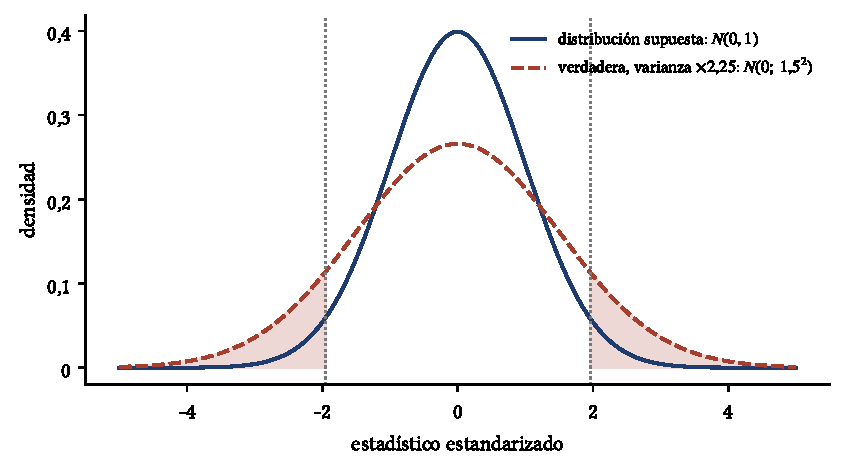
\includegraphics[width=0.78\linewidth]{graficos/cap16_fig_varianza_inducida.pdf}
\caption{Si el evento aumenta la varianza a $1{,}5^2$ pero la prueba supone $N(0,1)$, el área sombreada fuera de $\pm1{,}96$ es
la probabilidad real de rechazo bajo la hipótesis nula: 0,191 en lugar de 0,05.}
\label{fig:varinducida}
\end{figure}

\begin{observacion}
Las pruebas de este capítulo sirven para horizontes cortos. Para horizontes de meses o años, los errores del modelo de
rendimiento normal se acumulan, los rendimientos acumulados son muy asimétricos y la elección del modelo domina el
resultado (Barber y Lyon, 1997; Kothari y Warner, 2007).
\end{observacion}

% ---------------------------------------------------------------------
\section{Ejercicios resueltos}
% ---------------------------------------------------------------------

\begin{ejresuelto}{Los resultados de Facebook de julio de 2018}\label{ej:facebook}
\enunciado Facebook publicó sus resultados del segundo trimestre de 2018 después del cierre del 25 de julio. Estime los
rendimientos anormales con los tres modelos de rendimiento normal, contraste el del día 0 y calcule los CAR de
$(-1,+1)$, $(0,+5)$ y $(-5,+5)$. Verifique la Proposición~\ref{prop:ficticia}.

\solucion
\paso{Paso 1. El día 0 y el modelo de mercado.} El día 0 es el 26 de julio de 2018, y la ventana de estimación va del 28 de
julio de 2017 al 11 de julio de 2018. La acción cayó $18{,}96$\,\% y el mercado, $0{,}30$\,\%. Con $\hat\alpha=0{,}0212$ y
$\hat\beta=1{,}2789$:
\begin{align*}
  AR_0 &= -18{,}9609-0{,}0212-1{,}2789\times(-0{,}3032)\\
       &= -18{,}9609-0{,}0212+0{,}3878\\
       &= -18{,}5943\text{\,\%}.
\end{align*}

\paso{Paso 2. Su error estándar.} Con $s=1{,}3389$, $\hat\mu_m=0{,}0507$ y $S_{mm}=153{,}80$, por la
Proposición~\ref{prop:varar}:
\begin{align*}
  (R_{m0}-\hat\mu_m)^2 &= (-0{,}3032-0{,}0507)^2\\
                      &= 0{,}1253,\\
  1+\tfrac1{240}+\tfrac{0{,}1253}{153{,}80} &= 1+0{,}004167+0{,}000814\\
                                         &= 1{,}004981,\\
  \text{ee}(AR_0) &= 1{,}3389\sqrt{1{,}004981}\\
                  &= 1{,}3422,\\
  t &= \frac{-18{,}5943}{1{,}3422}\\
    &= -13{,}85 .
\end{align*}
El valor crítico de la $t_{238}$ al 5\,\% es 1,970: la caída es unas 14 desviaciones estándar de un día normal.

\paso{Paso 3. Comparación de modelos.}
\begin{center}\small
\begin{tabular}{@{}lrrrrrr@{}}
\toprule
Modelo & $s$ & $AR_0$ & $t$ & $CAR(-1,+1)$ & $CAR(0,+5)$ & $CAR(-5,+5)$ \\
\midrule
Mercado & 1,339 & $-18{,}59$ & $-13{,}85$ & $-18{,}42$ & $-18{,}11$ & $-15{,}76$ \\
Media constante & 1,685 & $-19{,}05$ & $-11{,}28$ & $-18{,}68$ & $-19{,}34$ & $-15{,}93$ \\
Ajustado por mercado & 1,352 & $-18{,}66$ & $-13{,}80$ & $-18{,}37$ & $-18{,}17$ & $-15{,}41$ \\
\bottomrule
\end{tabular}
\end{center}
Los tres modelos coinciden en la magnitud, porque el mercado casi no se movió ese día. La diferencia está en la
precisión: el modelo de mercado reduce la desviación estándar de 1,685 a 1,339 y aumenta el estadístico $t$. Ningún otro día
de la ventana es significativo; el mayor, $+2{,}10$\,\% el 2 de agosto, tiene $t=1{,}56$ (Figura~\ref{fig:facebook}).

\paso{Paso 4. La ficticia.} La regresión de la ventana de estimación más el día 0, con una ficticia del día 0, da $\hat\delta=-18{,}5943$
y ee $=1{,}3422$, idénticos a los pasos 1 y 2.

\paso{Paso 5. Una ventana de estimación contaminada.} La ventana incluye el caso Cambridge Analytica de marzo de 2018
(Ejercicio~\ref{ej:cambridge}). Excluyendo del 19 al 26 de marzo, $s$ baja a 1,2844 y $t$ sube a $-14{,}47$; la conclusión no cambia,
pero muestra que los días con eventos propios deben quitarse de la estimación.

\codigoweb{cap16_ej01}
\salidaR{cap16_ej01_R.txt}
\lectura{cap16_ej01}

\RvsPy La función \texttt{rendimientos\_normales} devuelve en ambos lenguajes el vector de $AR$ y la matriz $V$ completa del
Corolario~\ref{cor:varcar}, de modo que cualquier CAR se obtiene con $\boldsymbol\gamma'\mathbf{AR}$ y $\sqrt{\boldsymbol\gamma'V\boldsymbol\gamma}$. La
regresión con la ficticia se hace con \texttt{lm} en R y con álgebra matricial en Python. Los índices difieren en uno
(R empieza en 1), por eso el R imprime \texttt{t0 - 1} como posición.

\begin{figure}[ht]
\centering
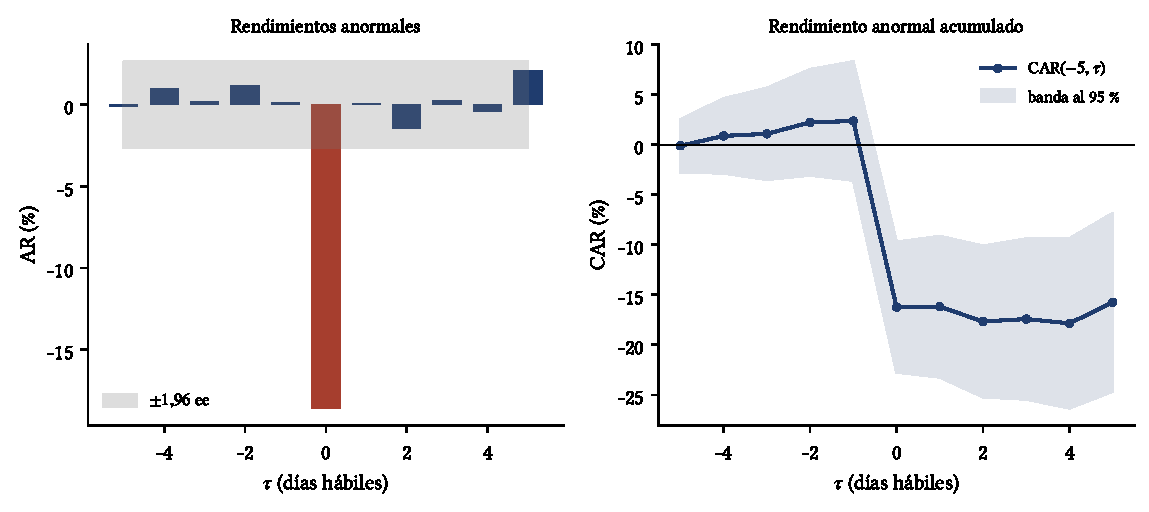
\includegraphics[width=\linewidth]{graficos/cap16_ej01_facebook.pdf}
\caption{Facebook alrededor del 26 de julio de 2018 (modelo de mercado). Izquierda: rendimientos anormales diarios con la
banda de $\pm1{,}96$ errores estándar. Derecha: CAR desde $\tau=-5$ con su banda al 95\,\%.}
\label{fig:facebook}
\end{figure}

\begin{conclusion}
El anuncio destruyó cerca del 18,6\,\% del valor de Facebook en un día, sin reversión en la semana siguiente. Cuando el
efecto es así de grande, el modelo de rendimiento normal casi no importa; importa cuando el efecto es pequeño, que es el caso
habitual.
\end{conclusion}
\end{ejresuelto}

\begin{ejresuelto}{Cambridge Analytica y el contagio}\label{ej:cambridge}
\enunciado El sábado 17 de marzo de 2018 se publicó que la consultora Cambridge Analytica había obtenido datos de millones de
usuarios de Facebook. Con el lunes 19 de marzo como día 0, mida el efecto en Facebook y en Apple, Amazon y Alphabet. ¿Hubo
contagio al resto del sector? Use la cartera de pares para la prueba conjunta.

\solucion
\paso{Paso 1. Efecto por empresa} (modelo de mercado).
\begin{center}\small
\begin{tabular}{@{}lrrrrrrr@{}}
\toprule
 & $\hat\beta$ & $AR_0$ & $t$ & $CAR(0,+1)$ & $t$ & $CAR(0,+5)$ & $t$ \\
\midrule
FB   & 1,235 & $-5{,}05$ & $-4{,}74$ & $-7{,}83$ & $-5{,}21$ & $-10{,}25$ & $-3{,}88$ \\
AAPL & 1,227 & 0,18 & 0,18 & $-0{,}08$ & $-0{,}06$ & 1,07 & 0,44 \\
AMZN & 1,071 & $-0{,}37$ & $-0{,}27$ & 1,98 & 1,05 & 1,67 & 0,50 \\
GOOG & 1,358 & $-1{,}27$ & $-1{,}46$ & $-1{,}69$ & $-1{,}39$ & $-2{,}98$ & $-1{,}39$ \\
\bottomrule
\end{tabular}
\end{center}
Facebook perdió un 10,2\,\% anormal en seis días; ninguno de los pares tiene un efecto significativo.

\paso{Paso 2. La prueba conjunta de los pares.} Los tres eventos tienen la misma fecha y sus residuos están
correlacionados (0,32, 0,30 y 0,47). La cartera igualmente ponderada da $CAR(0,+5)=-0{,}078$ con ee $=2{,}012$. La prueba ingenua,
que supone independencia, usa ee $=1{,}547$. El cociente es
\begin{align*}
  \frac{2{,}0118}{1{,}5467} &= 1{,}301,
\end{align*}
cercano al que predice la Proposición~\ref{prop:agrupado} con la correlación media $\bar\rho=0{,}361$ y $N=3$:
\begin{align*}
  \sqrt{1+(3-1)\times0{,}361} &= \sqrt{1{,}723}\\
                             &= 1{,}313 .
\end{align*}
Aquí no cambia la conclusión (no hay contagio), pero con muchas empresas y un efecto pequeño la prueba ingenua rechazaría
con demasiada frecuencia.

\paso{Paso 3. Facebook frente a sus pares.} El rendimiento de FB menos el de la cartera de pares, con el modelo de media, tiene
$CAR(0,+5)=-10{,}23$ y $t=-4{,}35$: el golpe fue propio de Facebook (Figura~\ref{fig:cambridge}).

\codigoweb{cap16_ej02}
\salidaR{cap16_ej02_R.txt}
\lectura{cap16_ej02}

\RvsPy La cartera se forma promediando los rendimientos fila por fila: \texttt{rowMeans} en R, \texttt{mean(1)} en Python. Los
residuos de la estimación quedan guardados en el componente \texttt{e} del resultado, lo que permite calcular su correlación
sin volver a estimar.

\begin{figure}[ht]
\centering
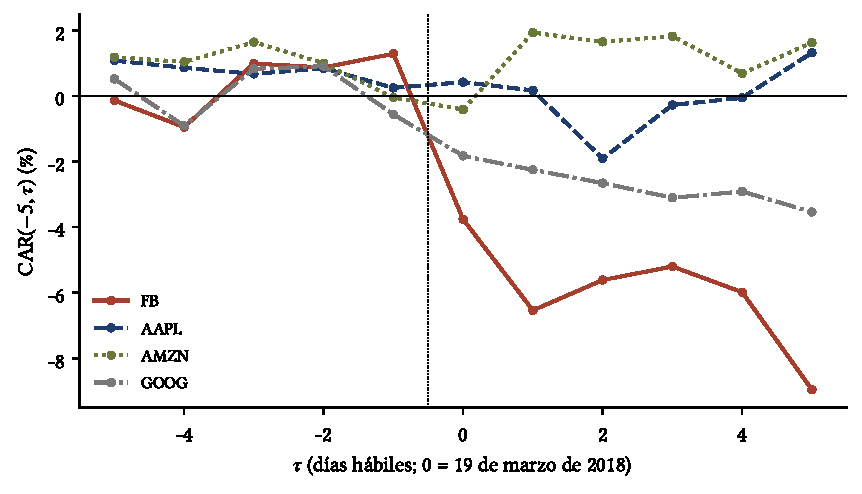
\includegraphics[width=0.8\linewidth]{graficos/cap16_ej02_cambridge.pdf}
\caption{CAR desde $\tau=-5$ de las cuatro empresas alrededor del 19 de marzo de 2018. Solo Facebook se separa de cero.}
\label{fig:cambridge}
\end{figure}

\begin{conclusion}
Cuando varios activos comparten la fecha del evento, la prueba correcta trata la cartera como una sola observación. El
escándalo afectó a Facebook y no al resto de las grandes tecnológicas.
\end{conclusion}
\end{ejresuelto}

\begin{ejresuelto}{Los anuncios del FOMC y el S\&P 500}\label{ej:fomc}
\enunciado Con las 40 reuniones programadas del FOMC de 2014 a 2018, estudie el S\&P 500 entre $\tau=-5$ y $+5$ del día del
comunicado. Use el modelo de media constante (el índice es el propio mercado), las cinco pruebas y la regresión con ficticias
de los días $-1$ y $0$ en toda la muestra.

\solucion
\paso{Paso 1. Rendimiento anormal medio por día.}
\begin{center}\small
\begin{tabular}{@{}rrrrrrr@{}}
\toprule
$\tau$ & $\overline{AR}$ & $J_1$ & Patell & BMP & Signo & $N^+/N$ \\
\midrule
$-2$ & $-0{,}218$ & $-1{,}75$ & $-1{,}83$ & $-2{,}17$ & $-2{,}53$ & 12/40 \\
$-1$ & 0,176 & 1,42 & 1,16 & 1,25 & 1,90 & 26/40 \\
0    & $-0{,}029$ & $-0{,}23$ & $-0{,}20$ & $-0{,}22$ & $-1{,}58$ & 15/40 \\
$+1$ & $-0{,}128$ & $-1{,}03$ & $-1{,}14$ & $-0{,}92$ & $-0{,}63$ & 18/40 \\
\bottomrule
\end{tabular}
\end{center}
El día del anuncio no hay efecto medio ($-0{,}03$\,\%; Corrado $=-0{,}92$). La víspera el índice subió $0{,}18$\,\% más que lo
normal, con 26 de 40 días positivos, pero no es significativo al 5\,\%. Los $CAAR$ de las ventanas $(-1,0)$, $(0,+5)$ y $(-5,+5)$
tampoco lo son ($J_1=0{,}84$, $-1{,}27$ y $-1{,}04$).

\paso{Paso 2. Interpretación de $\tau=-2$.} BMP y signo rechazan en $\tau=-2$. Pero se probaron 11 días: con 11 pruebas al 5\,\%,
la probabilidad de al menos un rechazo falso, si fueran independientes, es
\begin{align*}
  1-0{,}95^{11} &= 1-0{,}5688\\
               &= 0{,}431 .
\end{align*}
Un rechazo aislado en un día sin justificación económica previa no es evidencia convincente.

\paso{Paso 3. Regresión con ficticias.} En los 1\,258 días de 2014 a 2018, con errores de White:
\begin{align*}
  r_t = \underset{(0{,}0245)}{0{,}0216}+\underset{(0{,}1073)}{0{,}1986}\,D_t^{(-1)}-\underset{(0{,}1191)}{0{,}0067}\,D_t^{(0)} .
\end{align*}
La víspera del anuncio rinde 0,20 puntos más que un día normal ($t=1{,}85$). Lucca y Moench (2015) documentaron un
\emph{drift} previo al FOMC mucho mayor entre 1994 y 2011, concentrado en las 24 horas antes del comunicado; con cierres
diarios y estos cinco años el efecto es menor y no significativo al 5\,\%. Además, la desviación estándar del día del anuncio
(0,747) es \emph{menor} que la de los días normales (0,841): no hay varianza inducida (Figura~\ref{fig:fomc}).

\codigoweb{cap16_ej03}
\salidaR{cap16_ej03_R.txt}
\lectura{cap16_ej03}

\RvsPy Las fechas se localizan con \texttt{match} en R y con \texttt{np.where} en Python. Como el día 0 de cada evento tiene su
propia ventana de estimación, las 40 estimaciones se hacen con \texttt{lapply} o con una comprensión de listas, y los $AR$ se
apilan en una matriz $40\times11$. Los errores de White se calculan a mano, $(X'X)^{-1}X'\mathrm{diag}(e^2)X(X'X)^{-1}$.

\begin{figure}[ht]
\centering
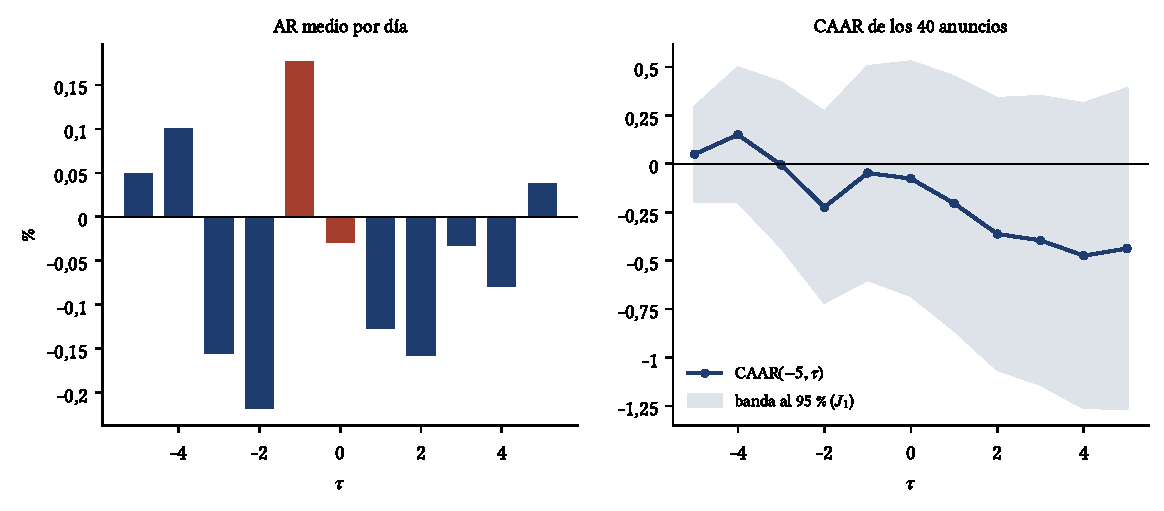
\includegraphics[width=\linewidth]{graficos/cap16_ej03_fomc.pdf}
\caption{S\&P 500 alrededor de los 40 comunicados del FOMC de 2014 a 2018. Izquierda: rendimiento anormal medio por día (en
rojo, la víspera y el día del anuncio). Derecha: CAAR con la banda al 95\,\% de $J_1$.}
\label{fig:fomc}
\end{figure}

\begin{conclusion}
Entre 2014 y 2018 los comunicados del FOMC no movieron el S\&P 500 en promedio. Un efecto nulo es un resultado tan válido
como uno significativo; lo importante es no buscar día por día hasta encontrar un rechazo.
\end{conclusion}
\end{ejresuelto}

\begin{ejresuelto}{Tamaño y potencia de las pruebas}\label{ej:potencia}
\enunciado Repita el diseño de Brown y Warner (1985) con datos reales: forme 1\,000 muestras de $N=20$ eventos, cada uno una
acción elegida al azar entre las cuatro y una fecha al azar entre 1\,007 posibles. Agregue un rendimiento anormal
$\delta\in\{0;\ 0{,}5;\ 1;\ 2\}$\,\% al día 0 y calcule la frecuencia de rechazo al 5\,\% de cada prueba.

\solucion
\paso{Paso 1. Resultados.}
\begin{center}\small
\begin{tabular}{@{}rrrrrr@{}}
\toprule
$\delta$ (\%) & $J_1$ & Patell & BMP & Signo & Corrado \\
\midrule
0,0 & 0,053 & 0,060 & 0,066 & 0,042 & 0,057 \\
0,5 & 0,362 & 0,440 & 0,526 & 0,467 & 0,638 \\
1,0 & 0,930 & 0,964 & 0,937 & 0,940 & 0,992 \\
2,0 & 1,000 & 1,000 & 0,992 & 1,000 & 1,000 \\
\bottomrule
\end{tabular}
\end{center}

\paso{Paso 2. Tamaño.} Con $\delta=0$, todas rechazan cerca del 5\,\%. Con 1\,000 muestras, el error estándar de una frecuencia de
0,05 es
\begin{align*}
  \sqrt{\frac{0{,}05\times0{,}95}{1\,000}} &= \sqrt{0{,}0000475}\\
                                         &= 0{,}0069,
\end{align*}
así que el 6,6\,\% de BMP está algo por encima. Se debe a usar 1,96 en lugar del valor crítico de la $t_{19}$, que es 2,09; con
$N=20$ la diferencia importa.

\paso{Paso 3. Potencia.} Con $\delta=0{,}5$\,\%, la prueba de rangos de Corrado detecta el efecto en el 64\,\% de las muestras y
$J_1$ solo en el 36\,\%. La razón está en la distribución de los rendimientos anormales: su asimetría es 1,14 y sus colas son
pesadas. Las pruebas paramétricas pierden potencia con valores extremos, que inflan la varianza estimada; los rangos no se
ven afectados. Patell y BMP superan a $J_1$ porque ponderan más los activos menos volátiles (Figura~\ref{fig:potencia}).

\codigoweb{cap16_ej04}
\salidaR{cap16_ej04_R.txt}
\lectura{cap16_ej04}

\RvsPy Los generadores aleatorios de R y de NumPy son distintos, así que las mismas instrucciones darían muestras distintas.
Para reproducir los resultados exactamente en ambos lenguajes usamos un generador propio, el congruencial de Park y Miller
(1988), $x\leftarrow16\,807\,x \bmod (2^{31}-1)$. Los productos no pasan de $3{,}6\times10^{13}$, menos que $2^{53}$, de modo que la
aritmética de doble precisión de R es exacta. Ese generador sirve para enseñar, no para simulaciones serias, que deben usar
los generadores modernos de cada lenguaje. Los rendimientos anormales de las 4\,028 combinaciones posibles se calculan una
sola vez antes de la simulación.

\begin{figure}[ht]
\centering
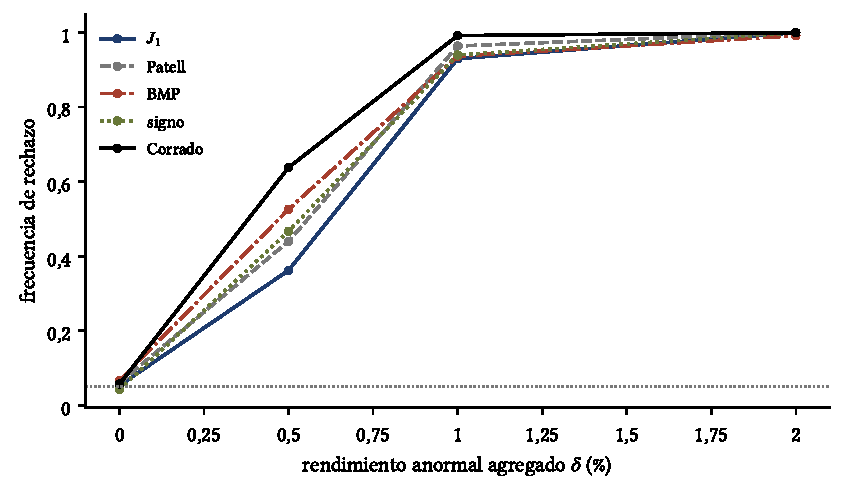
\includegraphics[width=0.78\linewidth]{graficos/cap16_ej04_potencia.pdf}
\caption{Frecuencia de rechazo al 5\,\% de cada prueba según el rendimiento anormal agregado, con 1\,000 muestras de 20 eventos.
La línea punteada marca el 5\,\% nominal.}
\label{fig:potencia}
\end{figure}

\begin{conclusion}
Con rendimientos diarios de acciones individuales, todas las pruebas tienen el tamaño correcto, pero la de rangos es
claramente más potente para efectos pequeños. Conviene informar al menos una prueba paramétrica y una no paramétrica.
\end{conclusion}
\end{ejresuelto}

\begin{ejresuelto}{Varianza inducida por el evento}\label{ej:varinducida}
\enunciado (a) Repita la simulación del Ejercicio~\ref{ej:potencia}, pero ahora el evento multiplica por 2,25 la varianza del
día 0: a cada $AR$ se le suma un ruido normal de varianza $1{,}25\,\hat\sigma_i^2$. (b) Estudie el cambio porcentual del VIX
alrededor de los anuncios del FOMC.

\solucion
\paso{Paso 1. La simulación.}
\begin{center}\small
\begin{tabular}{@{}rrrrrr@{}}
\toprule
$\delta$ (\%) & $J_1$ & Patell & BMP & Signo & Corrado \\
\midrule
0,0 & 0,216 & 0,217 & 0,078 & 0,057 & 0,143 \\
1,0 & 0,823 & 0,861 & 0,681 & 0,475 & 0,782 \\
\bottomrule
\end{tabular}
\end{center}
Sin efecto en la media, $J_1$ y Patell rechazan el 22\,\% de las veces, muy cerca del 19,1\,\% que predice la
Proposición~\ref{prop:varinducida}. BMP se mantiene cerca del 5\,\% (el exceso, como antes, se debe al valor crítico) y la prueba
del signo también. La de rangos, que era la mejor sin varianza inducida, rechaza el 14\,\%: los valores extremos del día 0
obtienen rangos extremos con más frecuencia de la que supone su denominador. Con $\delta=1$\,\%, la potencia de BMP (0,68) es
menor que la de $J_1$, pero esta última se logra a costa de rechazar demasiado bajo la nula.

\paso{Paso 2. El VIX y el FOMC.}
\begin{center}\small
\begin{tabular}{@{}rrrrrr@{}}
\toprule
$\tau$ & $\overline{AR}$ (\%) & $J_1$ & BMP & $N^+/N$ & $\widehat{\Var}(SAR)$ \\
\midrule
$-2$ & 3,54 & 2,80 & 2,67 & 25/40 & 0,969 \\
$-1$ & $-1{,}68$ & $-1{,}33$ & $-1{,}34$ & 18/40 & 0,840 \\
0    & $-1{,}48$ & $-1{,}17$ & $-1{,}27$ & 19/40 & 0,970 \\
$+3$ & 1,66 & 1,31 & 0,80 & 21/40 & 4,066 \\
\bottomrule
\end{tabular}
\end{center}
El VIX tiende a bajar la víspera y el día del anuncio: $CAAR(-1,0)=-3{,}16$\,\%, con $J_1=-1{,}76$ y BMP $=-2{,}02$, en el límite de la
significancia. La varianza de corte transversal de los $SAR$ en el día 0 es 0,97, cercana a uno: los anuncios no aumentaron la
dispersión. En $\tau=+3$ es 4,07 por un solo evento: el 5 de febrero de 2018, tres días hábiles después del comunicado del 31
de enero, el VIX subió 76,8\,\% en logaritmos, en el desplome de los productos de volatilidad inversa. Ahí $J_1$ (1,31) y BMP (0,80)
difieren justamente porque BMP usa esa dispersión en el denominador. El rechazo en $\tau=-2$ tiene el mismo problema de
pruebas múltiples que en el Ejercicio~\ref{ej:fomc} (Figura~\ref{fig:vix}).

\codigoweb{cap16_ej05}
\salidaR{cap16_ej05_R.txt}
\lectura{cap16_ej05}

\RvsPy Los ruidos normales se generan con el método de Box y Muller:
\[
  z=\sqrt{-2\ln u_1}\,\cos(2\pi u_2),
\]
a partir de dos uniformes del generador de Park y Miller; así R y Python reciben los mismos
números. En R, la matriz \texttt{s[, 1:2]} de pares (acción, fecha) sirve directamente como índice de la matriz \texttt{AR0}.

\begin{figure}[ht]
\centering
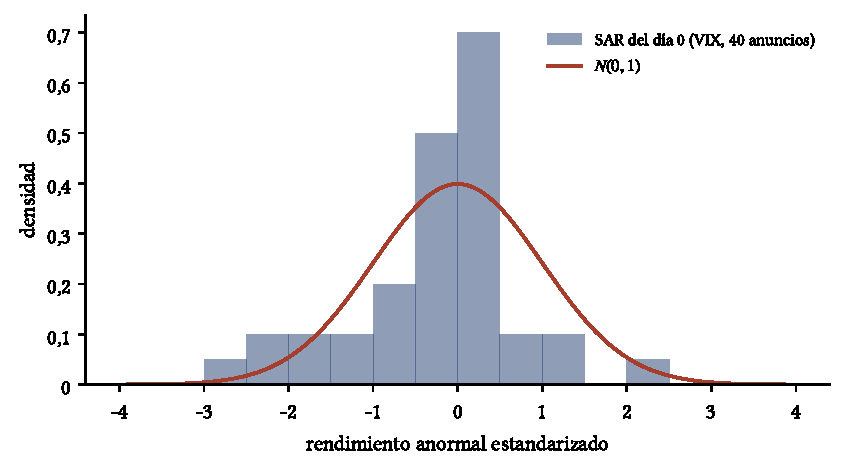
\includegraphics[width=0.78\linewidth]{graficos/cap16_ej05_vix.pdf}
\caption{Histograma de los rendimientos anormales estandarizados del VIX en el día de los 40 anuncios del FOMC, con la
densidad $N(0,1)$ que suponen las pruebas.}
\label{fig:vix}
\end{figure}

\begin{conclusion}
Cuando un evento puede aumentar la volatilidad, que es lo habitual en anuncios de resultados o fusiones, las pruebas que usan
la varianza de la ventana de estimación rechazan demasiado. BMP es la opción paramétrica segura, y la de rangos debe
interpretarse con cuidado.
\end{conclusion}
\end{ejresuelto}

% ---------------------------------------------------------------------
\section{Ejercicios propuestos}
% ---------------------------------------------------------------------

\begin{enumerate}[label=\textbf{\thechapter.\arabic*},leftmargin=*,itemsep=6pt]
  \item Con $L_1=240$, $s=1{,}2$, $R_{m0}=2$, $\hat\mu_m=0{,}05$ y $S_{mm}=240$, calcule el error estándar de $AR_0$ en el modelo de
  mercado. \textit{Respuesta: el factor es $1{,}02001$; ee $=1{,}2119$.}

  \item Con $N=30$ eventos, $L_1-2=238$ y $\sum_iSAR_i=12$, calcule el estadístico de Patell. \textit{Respuesta: $12/\sqrt{30{,}254}=2{,}182$.}

  \item Diez empresas con el mismo día de evento tienen rendimientos anormales con correlación $0{,}3$. ¿Por qué factor subestima
  la prueba ingenua el error estándar del promedio? \textit{Respuesta: $\sqrt{1+9\times0{,}3}=1{,}924$.}

  \item Demuestre que en el modelo ajustado por mercado, con $\sigma^2$ estimada con la varianza de $R_i-R_m$ en la ventana de estimación,
  $\Var(CAR(\tau_1,\tau_2))=(\tau_2-\tau_1+1)\sigma^2$, y explique por qué no hay término de error de estimación.

  \item Demuestre que, bajo la hipótesis nula y con $AR_i$ independientes y de mediana cero, el estadístico del signo converge a
  $N(0,1)$.

  \item \emph{(Simulación.)} Repita el Ejercicio~\ref{ej:potencia} con $N=50$. ¿Se reduce el exceso de rechazo de BMP? ¿Cambia el orden de
  potencia de las pruebas?

  \item \emph{(Con datos de la BVL.)} Elija un anuncio relevante de una empresa peruana (por ejemplo, un cambio de calificación
  crediticia o un anuncio de dividendos) y estudie su efecto con el índice S\&P/BVL Perú General como mercado. Discuta el
  problema de la negociación poco frecuente: ¿qué pasa con $\hat\beta$ si la acción no cotiza todos los días? (Scholes y Williams, 1977.)

  \item \emph{(Con datos.)} Repita el Ejercicio~\ref{ej:facebook} con una ventana de estimación de 120 días, $\tau=-130,\dots,-11$. ¿Cambian
  $\hat\beta$, $s$ y el estadístico $t$?
\end{enumerate}

% ---------------------------------------------------------------------
\section{Resumen de fórmulas}
% ---------------------------------------------------------------------

\begin{table}[H]
\centering\small
\begin{tabular}{@{}ll@{}}
\toprule
Concepto & Fórmula \\
\midrule
Rendimiento anormal & $AR_{i\tau}=R_{i\tau}-\hat\alpha_i-\hat\beta_iR_{m\tau}$;\quad $CAR_i(\tau_1,\tau_2)=\sum_{\tau=\tau_1}^{\tau_2}AR_{i\tau}$ \\
Varianza del AR & $\sigma^2\bigl[1+\frac1{L_1}+\frac{(R_{m\tau}-\hat\mu_m)^2}{S_{mm}}\bigr]$ \\
Varianza del vector AR & $V_i=\sigma^2[I+X^*(X'X)^{-1}X^{*\prime}]$;\quad $\Var(CAR)=\boldsymbol\gamma'V_i\boldsymbol\gamma$ \\
Ficticia & $R_{it}=\alpha_i+\beta_iR_{mt}+\delta D_t+u_t$;\quad $\hat\delta=AR_{i\tau}$ \\
$J_1$ & $\overline{AR}/\sqrt{\sum_i\hat\sigma_i^2/N^2}$ \\
Patell & $\sum_iSAR_i/\sqrt{\sum_ig/(g-2)}$ \\
BMP & $\overline{SAR}/(s_{SAR}/\sqrt N)$ \\
Signo & $(N^+-N/2)/\sqrt{N/4}$ \\
Eventos simultáneos & $\Var(\overline{AR})=\frac{\sigma^2}{N}[1+(N-1)\rho]$ \\
Varianza inducida & $J_1$, Patell $\to N(0,c)$;\quad BMP $\to N(0,1)$ \\
\bottomrule
\end{tabular}
\caption{Fórmulas principales del Capítulo 16.}
\end{table}

\section*{Referencias}
\begin{itemize}[leftmargin=*]
  \item Barber, B. M. y Lyon, J. D. (1997). Detecting long-run abnormal stock returns: The empirical power and specification
        of test statistics. \emph{Journal of Financial Economics}, 43(3), 341--372.
  \item Boehmer, E., Musumeci, J. y Poulsen, A. B. (1991). Event-study methodology under conditions of event-induced
        variance. \emph{Journal of Financial Economics}, 30(2), 253--272.
  \item Brown, S. J. y Warner, J. B. (1985). Using daily stock returns: The case of event studies. \emph{Journal of Financial
        Economics}, 14(1), 3--31.
  \item Campbell, J. Y., Lo, A. W. y MacKinlay, A. C. (1997). \emph{The Econometrics of Financial Markets}, cap. 4. Princeton
        University Press.
  \item Corrado, C. J. (1989). A nonparametric test for abnormal security-price performance in event studies. \emph{Journal
        of Financial Economics}, 23(2), 385--395.
  \item Fama, E. F., Fisher, L., Jensen, M. C. y Roll, R. (1969). The adjustment of stock prices to new information.
        \emph{International Economic Review}, 10(1), 1--21.
  \item Kothari, S. P. y Warner, J. B. (2007). Econometrics of event studies. En B. E. Eckbo (ed.), \emph{Handbook of
        Corporate Finance}, vol. 1, 3--36. Elsevier.
  \item Lucca, D. O. y Moench, E. (2015). The pre-FOMC announcement drift. \emph{Journal of Finance}, 70(1), 329--371.
  \item MacKinlay, A. C. (1997). Event studies in economics and finance. \emph{Journal of Economic Literature}, 35(1), 13--39.
  \item Park, S. K. y Miller, K. W. (1988). Random number generators: Good ones are hard to find. \emph{Communications of the
        ACM}, 31(10), 1192--1201.
  \item Patell, J. M. (1976). Corporate forecasts of earnings per share and stock price behavior: Empirical tests.
        \emph{Journal of Accounting Research}, 14(2), 246--276.
  \item Scholes, M. y Williams, J. (1977). Estimating betas from nonsynchronous data. \emph{Journal of Financial Economics},
        5(3), 309--327.
\end{itemize}
